% PLEASE USE THIS FILE AS A TEMPLATE
% Check file iosart2c.tex for more examples
%
% Journal:
%   Journal of Ambient Intelligence and Smart Environments (jaise)
%   Web Intelligence and Agent Systems: An International Journal (wias)
%   Semantic Web: Interoperability, Usability, Applicability (SW)
% IOS Press
% Latex 2e

% options: jaise|wias|sw
% add. options: [seceqn,secfloat,secthm,crcready,onecolumn]


\documentclass[sw]{iosart2c}

%\documentclass[sw]{iosart2c}
%\documentclass[wias]{iosart2c}
%\documentclass[jaise]{iosart2c}

\usepackage[T1]{fontenc}
\usepackage{times}%
\usepackage{natbib}% for bibliography sorting/compressing
%\usepackage{amsmath}
%\usepackage{endnotes}
\usepackage{graphicx}
%\usepackage{tikz}
%\usetikzlibrary{snakes,arrows,shapes}

%%%%%%%%%%% Put your definitions here

% \bibliographystyle{plain} 
\bibliographystyle{unsrt} 

%%%%%%%%%%% End of definitions

\pubyear{0000}
\volume{0}
\firstpage{1}
\lastpage{1}

\begin{document}

\newcommand{\url}[1]{#1}

\begin{frontmatter}

%\pretitle{}
\title{The ChEMBL database as Linked Open Data}
\runningtitle{ChEMBL-RDF}
%\subtitle{}

%\review{}{}{}


% For one author:
\author[A]{\fnms{Egon} \snm{Willighagen}\thanks{Corresponding author.\\ E-mail: egon.willighagen@maastrichtuniversity.nl.}}
\runningauthor{E.L. Willighagen et al.}
% Two or more authors (order to be determined):
\author[A]{\fnms{Andra} \snm{Waagmeester}}
\author[B]{\fnms{Ola} \snm{Spjuth}},
\author[C]{\fnms{Peter} \snm{Ansell}},
\author[D]{\fnms{Antony} \snm{Williams}},
\author[D]{\fnms{Valery} \snm{Tkachenko}},
\author[E]{\fnms{Janna} \snm{Hastings}},
\author[F]{\fnms{John} \snm{Overington}},
\author[F]{\fnms{Anna} \snm{Gaulton}},
\author[F]{\fnms{Mark} \snm{Davies}},
\author[G]{\fnms{Bin} \snm{Chen}},
\author[G]{\fnms{David} \snm{Wild}}

\address[A]{Department of Bioinformatics - BiGCaT, Maastricht University, P.O. Box 616, UNS50 Box 19, NL-6200 MD, Maastricht, The Netherlands}
\address[B]{Department of Pharmaceutical Biosciences, Uppsala University, PO Box 591, SE-751 24, Uppsala, Sweden}
\address[C]{University of Queensland, St Lucia, Qld 4072, Australia}
\address[D]{Royal Society of Chemistry, 904 Tamaras Circle, Wake Forest, NC 27587, U.S.A.}
\address[E]{Chemoinformatics and Metabolism, European Bioinformatics Institute, POSTAL CODE, Hinxton, United Kingdom}
\address[F]{EMBL-European Bioinformatics Institute, Wellcome Trust Genome Campus, Hinxton, Cambridgeshire, CB10 1SD, United Kingdom}
\address[G]{School of Informatics and Computing, Indiana University, Bloomington, IN, U.S.A.}

\begin{abstract}
Making data available as Linked Data using RDF is advantageous because it promotes integration with other web resources.
RDF documents can natively link to related data, and others can link back using URIs. RDF makes the data machine-readable,
using extensible vocabularies for additional information. This combination provides a new, open, interface for scientists to use ChEMBL.
This paper describes the continued conversion of data from the ChEMBL database into RDF triples.
This updated version of ChEMBL-RDF now uses recently introduced ontologies, including CHEMINF and CiTO,
exposes more information from the database, and is now available as dereferencable, Linked Data.
To demonstrate the new features, we present new use cases showing the benefits of integration with
other web resources using semantic web technologies.
\end{abstract}

\begin{keyword}
% \sep 
Resource Description Framework, ChEMBL
\end{keyword}

\end{frontmatter}

%%%%%%%%%%% The article body starts:

\section{Introduction}\label{s1}


The current scientific data deluge, in which datasets are growing faster than scientists can analyse and 
curate them, provides several new challenges for information systems. Scientists wish to 
discover new, unique, and significant patterns in datasets, which explaining biological 
phenomena not yet understood. This process requires integration of datasets that are both 
sparse, and growing independent of one another. The discovery of new patterns showing the 
causes and effects of various biological phenomena is beyond the scope of single datasets.
For example, systems biologists integrate micro-array differential expression datasets to 
biological pathways, using various other datasets to provide evidence for the links~\cite{}. 
Another prominent example is drug discovery where a new unique chemical entity is discovered 
based on descriptions of its biological properties. This process requires the effective 
linkage of many scientific datasets~\cite{Samwald2011,OpenPHACTS}.

ChEMBL contains descriptions for biological activities involving over a million chemical 
entities, extracted from literature. This provides a unique resource for drug researchers~\cite{Gaulton2012,Warr2009}.
It is updated on a fairly frequent basis as the existing data is further curated and new data is added. 
The ChEMBL dataset is available for download and can be browsed using a web interface. 
The former requires scientists to import the data into a relational database, while the 
latter limits the machine access to the data. Two independent teams have previously mapped 
the ChEMBL dataset to RDF, Chem2Bio2RDF~\cite{Chen2010} and ChEMBL-RDF~\cite{Willighagen2011}.

This paper presents the current state of the ChEMBL-RDF dataset, details of the latest structures
and ontologies used to map version 13 of ChEMBL to RDF, along with new example use cases, showing 
links to other datasets using their RDF URIs to further support research in the life sciences.

\section{Methods}\label{s2}

The ChEMBL version used in this paper is ChEMBL 13, which was released on 29 February 2012.
The SQL datadump provided by EMBL was inserted into a local MySQL database. A set of SQL queries 
were then executed to generate RDF files using a set of PHP scripts. These scripts are Open Source 
and are available from the source code hosting service, GitHub~\citep{ChEMBLRDFGitHub}. This process 
has been outlined in a best practices note by the W3C Health Care and Life Sciences XXX Working Group~\cite{Marshall2012}.

In the previous RDF conversion the RDF triples in ChEMBL-RDF were represented using properties and c
lasses from a custom, ad-hoc ontology~\cite{Willighagen2011}. The current version used community-proposed
ontologies, making the RDF more interoperable. The ChEMBL-RDF 13 dataset uses ontology
standards such as the Bibliography Ontology~\cite{Giasson2011} and the Citation Typing Ontology~\cite{Hastings2011} for literature
references, and domain ontologies like the Protein Ontology\cite{Sidhu2006} and the Chemical Information
Ontology\cite{Hastings2011}. Throughout this paper, various shorthand prefixes are used to denote different ontology 
namespaces to simplify the RDF examples. These prefixes are outlined in Table~\ref{namespaces}.

\begin{table*}
\caption{Prefixes and their matching namespaces used in this paper.} \label{namespaces}
\begin{tabular}{ll}
\hline
\multicolumn{2}{l}{\textbf{Common Vocabularies}} \\
bibo    & Bibliography Ontology~\cite{Giasson2011} \\
        & http://purl.org/ontology/bibo/ \\
chebi   & Chemical Entities of Biological Interest~\cite{DeMatos2010} \\
        & http://purl.org/obo/owl/CHEBI\# \\
cheminf & Chemical Information Ontology~\cite{Hastings2011} \\
        & http://semanticscience.org/resource/ \\
cito    & Citation Typing Ontology~\cite{Shotton2010} \\
        & http://purl.org/spar/cito/ \\
obo / pro & OBO \& PRotein Ontology~\cite{Sidhu2006} \\
          & http://purl.obolibrary.org/obo/ \\

\multicolumn{2}{l}{\textbf{ChEMBL-RDF Namespace}} \\
chembl & http://rdf.farmbio.uu.se/chembl/onto/\# \\

\multicolumn{2}{l}{\textbf{ChEMBL-RDF Prefixes }}\\
act    & http://data.kasabi.com/dataset/chembl-rdf/activity/ \\
assay  & http://data.kasabi.com/dataset/chembl-rdf/assay/ \\
mol    & http://data.kasabi.com/dataset/chembl-rdf/molecule/ \\
res    & http://data.kasabi.com/dataset/chembl-rdf/resource/ \\
\hline
\end{tabular}
\end{table*}

To expose that ChEMBL-RDF data two approaches have been adopted. First, a SPARQL end point
hosted at Uppsala University, using the Open Source Virtuoso software. Use is free, but the
querying is capped, based on the estimated computational effort. Second, resources have
been made dereferencable using the Kasabi platform~\cite{kasabi}. The Kasabi hosting provides a SPARQL
end point which requires a user account. A user account can be free for casual usage, or paid for consistent usage.

Although many parts of the ChEMBL-RDF 13 dataset now use community based ontologies, some 
terms from the previous ad-hoc ontology are still used. These terms were created under the 
URI namespace \textit{http://rdf.farmbio.uu.se/chembl/onto/\#}, and are referenced here using the
prefix: \textit{chembl}.

%As a method to further test the access and possibilities of this Linked Data version of
%ChEMBL,  new uses cases have been developed for this paper.

\section{Results}\label{s3}

We here present the updated ChEMBL-RDF, including a description of the mapping process 
and the identification of links to other datasets.

\subsection{ChEMBL-RDF}

\subsubsection{Data Structure}

For each of the common resource classes, a triple pattern was defined, following the
data available in the relational database. Figure~\ref{f1} shows how the various resource
classes are linked together. This section will show how data in the ChEMBL database
is exposed at an triple level.

\begin{figure}[t]
\includegraphics[width=0.45\textwidth]{figs/relations}
\caption{The various resource types found in the ChEMBL triples. Some entities are subclasses
of common classes, while others are instances.}\label{f1}
\end{figure}

The core concept in the ChEMBL database is that of the biological activity. This
is the type of information that the ChEMBL database extracts from literature.
In ChEMBL-RDF activities are mostly represented using the custom ChEMBL-RDF vocabulary, where the
type, fields and links to other resources are using the \textit{chembl}
namespace. While ChEMBL provides both the original activities as found in literature
and standardized values allowing comparison between studies, the triples only
make the latter available. The CiTO ontology is used to point to the paper from
which the data was extracted.

\begin{footnotesize}
\begin{verbatim}
act:a31863
 a       chembl:Activity ;
 cito:citesAsDataSource
  res:r6424 ;
 chembl:forMolecule mol:m180094 ;
 chembl:onAssay assay:a54505 ;
 chembl:relation ">" ;
 chembl:standardUnits
  "nM" ;
 chembl:standardValue
  "100000"^^xsd:float ;
 chembl:type "IC50" .
\end{verbatim}
\end{footnotesize}

More than five thousand different activity types are captured by the ChEMBL database.
The top five types are Potency (43\%), IC50 (13\%), MIC (4.6\%), Inhibition (3.7\%),
and Ki (3.6\%). The activity types in ChEMBL-RDF are currently not available as, or
using, an ontology.

The activities themselves are measured against assays, which make up a second important
resource type. Various assay types are found in the database: chembl:ADMET, chembl:Binding,
chembl:Functional, chembl:Property, and chembl:Unassigned. The assay information link
activities to a target (see below) and has a short description. The confidence information
assigned by the ChEMBL is exposed too, and was previously used to improve activity
prediction using Bayesian statistics~\cite{Willighagen2011}.

\begin{footnotesize}
\begin{verbatim}
assay:a17
 a chembl:Assay ;
 cito:citesAsDataSource
  res:r11347 ;
 chembl:hasAssayType chembl:ADMET ;
 chembl:hasConfScore "7"^^xsd:int ;
 chembl:hasDescription
  "Inhibition of ... hydroxylase" ;
 chembl:hasTarget target:t100122 .
\end{verbatim}
\end{footnotesize}

The assays measure activities against particular biological targets. The ChEMBL database
recognizes various types: pro:PR\_0000001, chembl:ADMET, chembl:CELL-LINE,
chembl:NUCLEIC-ACID, chembl:ORGANISM, chembl:SUBCELLULAR, chembl:TISSUE,
chembl:UNCHECKED, and chembl:UNKNOWN. The latter two are currently defined as
explicit types.

\begin{footnotesize}
\begin{verbatim}
target:t1
 a chembl:Target ;
 rdfs:subClassOf pro:PR_000000001 ;
 rdfs:label "Glucoamylase" , 
  "Maltase-glucoamylase, intestinal" ;
 dc:identifier "uniprot:O43451" ,
   "3.2.1.3" ;
 dc:title "Maltase-glucoamylase" ;
 chembl:classL1 "Enzyme" ;
 chembl:hasDescription
  "Maltase-glucoamylase, intestinal" ;
 chembl:hasKeyword "Glycosidase" , 
  "Membrane" , "Sulfation" ;
 chembl:organism "Homo sapiens" .
\end{verbatim}
\end{footnotesize}

For drug discovery, the drugs themselves are the main topic of study.
ChEMBL contains many different drug types, mostly small molecules,
but also peptides, proteins, antibodies, oligosaccharides, oligonucleotides, and
even cells. All compounds are represented as classes, following
the design of the CHEMINF ontology. These entities do not have a common
superclass in common, but can easily be identified as having the 
the role of being a drug. This is triplified using the OBO and ChEBI
ontologies:

\begin{footnotesize}
\begin{verbatim}
mol:m4 obo:has_role chebi:CHEBI_23888 .
\end{verbatim}
\end{footnotesize}

The entity typing is expressed
by subclassing other classes. For example, proteins subclass the
Protein concept from the PRotein Ontology (PR\_000000001), small
molecules subclass the Chemical Entity concept from the CHEMINF
ontology (CHEMINF\_000000), and oligosaccharides and oligonucleotides
subclass their respective matches in the CHEBI ontology (CHEBI\_50699
and CHEBI\_7754). For each drug compound the name and synonyms are
provided as labels. When InChI and InChIKeys are available for a drug, then these are
provided via the CHEMINF formalism (here abbreviated):

\begin{footnotesize}
\begin{verbatim}
mol:m41
 rdfs:label "ChEMBL406142" , 
   "Bis(3-[1 .... yl]-propionamide)" ;
 rdfs:subClassOf cheminf:CHEMINF_000000 ;
 cheminf:CHEMINF_000200
  m41:inchikey , m41:smiles , m41:inchi ;

m41:inchikey
 a cheminf:CHEMINF_000059 ;
 cheminf:SIO_000300
   "LMCOMIDLRGMFCZ-RIPOXUOASA-N" .

m41:smiles
 a cheminf:CHEMINF_000018 ;
 cheminf:SIO_000300
  "CC(C)C[C@@H]1N2C= .... O)C7=O)NC1=O)C2=O" .

m41:inchi
 a cheminf:CHEMINF_000113 ;
 cheminf:SIO_000300
  "InChI=1S/C82H102N .... 66+,67+,68+/m1/s1" .

chemblid:ChEMBL406142
 owl:equivalentClass mol:m41 .
\end{verbatim}
\end{footnotesize}

For small molecules, molecular properties are often available from ChEMBL, and as of ChEMBL-RDF 13
these too are exposed in triple format. Like the InChI and InChIKey, these are provided using the
CHEMINF ontology approach. Here is, for example, the ALogP value:

\begin{footnotesize}
\begin{verbatim}
mol:m1
 cheminf:CHEMINF_000200 m1:alogp .

m1:alogp
 a cheminf:CHEMINF_000305 ;
 cheminf:SIO_000300
  "3.344"^^xsd:double .
\end{verbatim}
\end{footnotesize}

For documents little information is replicated from the database, taking advantage
of PubMed Identifiers (PMIDs) and Digital Object Identifiers (DOIs). URIs for the
latter can be resolved online, providing curated information on the identified
documents. For each paper, basic properties are provided using the BIBO
ontology:

\begin{footnotesize}
\begin{verbatim}
journal:j6c706049c2e08871b7c46a6528065736
 a bibo:Journal ;
 dc:title "J. Med. Chem." .

res:r1
 a bibo:Article ;
 dc:date "2004" ;
 dc:isPartOf
  journal:j6c706049c2e08871b7c46a6528065736 ;
 bibo:issue "1" ;
 bibo:pageEnd "9" ;
 bibo:pageStart "1" ;
 bibo:pmid "14695813" ;
 bibo:volume "47" .
\end{verbatim}
\end{footnotesize}

\subsubsection{Data Statistics}

\# triples
\# links out
\# problems

The full set of triples are available from the website http://semantics.bigcat.unimaas.nl/chembl12/.

FIXME!

In contrast to earlier releases of ChEMBL-RDF, it now contains the chemical properties
provided by the ChEMBL database as calculated by ACD/Labs and XXXXX. The data includes
chemical properties like polar surface area, pKa and logP, counts for hydrogen bond donor
and acceptor, and rotational bonds. This data is provided for XXXXX structures.

\subsubsection{Data Statistics and Validation}

Each release of the ChEMBL database is accompanied by set of release counts, which help 
provide a concise content overview of the release in question. The ChEMBL 13 release counts
are as follows:

\begin{itemize}
  \item 8,845 targets
  \item 1,143,682 distinct molecules
  \item 6,933,068 activities
  \item 617,681 assays
  \item 44,682 documents
\end{itemize}

These counts are important as firstly they show continued growth in ChEMBL data, as seen 
in all previous releases. Secondly, these counts can help validate any transformations, 
which have been applied to the relational data model traditionally used to store the ChEMBL 
data. The following SPARQL queries attempt to provide a high level validation of the 
ChEMBL-RDF by regenerating the ChEMBL 13 release statistics.

The following SPARQL query returns 8,845 ChEMBL targets:
     
\begin{tiny}
\begin{verbatim}
select count(*) WHERE {
  ?s ?p chembl:Target .
}
\end{verbatim}
\end{tiny}

The following SPARQL query returns 1,143,682 ChEMBL molecules:

%Mark Davies notes:
%NOTE: Full set of ChEMBL molecules have been created by querying molecule\_dictionary table
%NOTE: I have added extra triple for each molecule: <http://data.kasabi.com/dataset/chembl-rdf/13/molecule/m1> <http://www.w3.org/1999/02/22-rdf-syntax-ns#type> <http://rdf.farmbio.uu.se/chembl/onto/#Molecule> .
%NOTE: Modified molecule compound structure can be queried here: https://wwwdev.ebi.ac.uk/chembl/sparql

\begin{tiny}
\begin{verbatim}
select count(*) WHERE {
  ?s ?p chembl:Molecule .
}
\end{verbatim}
\end{tiny}

The following SPARQL query returns 617,681 ChEMBL assays:

\begin{tiny}
\begin{verbatim}
select count(*) WHERE {
  ?s ?p chembl:Assay .
}
\end{verbatim}
\end{tiny}

The following SPARQL query returns the 6,933,068 ChEMBL activities:

\begin{tiny}
\begin{verbatim}
select count(*) WHERE {
  ?s ?p chembl:Activity .
}
\end{verbatim}
\end{tiny}

The following SPARQL query returns the 44,681 ChEMBL documents. This is 1 less than appears 
in ChEMBL 13 release notes, as it does not include doc\_id -1, which refers to the 
unpublished dataset.

\begin{tiny}
\begin{verbatim}
select count(*) WHERE {
  ?s ?p bibo:Article .
}
\end{verbatim}
\end{tiny}

Recreation of the ChEMBL release statistics, by querying the ChEMBL-RDF with SPARQL 
provides end users with high degree of confidence that the ChEMBL-RDF contains same 
core content as source relational database. 


\subsection{Linked Open Data}

To integrate ChEMBL-RDF with other RDF versions of scientific datasets, we link out to various resources.
These links are shown in Figure~\ref{2}. Triples for compounds link out to ChemSpider 
using the complementary index and OpenMolecules RDF using InChI values. Protein links are given to Bio2RDF
using the Uniprot identifier. Literature references are directed to CrossRef and Bio2RDF 
using the DOIs and PubMed identifiers, respectively.

\begin{figure}[t]
\includegraphics[width=0.45\textwidth]{figs/lodgraph}
\caption{The links out of the ChEMBL-RDF data into the Linked Open Data cloud.
Edges are labeled by the predicates making the links.}\label{2}
\end{figure}

\subsubsection{Linking out to Bio2RDF}

The Bio2RDF project provides both resolvable Linked Data URIs using a generic Linked Data
server~\cite{Ansell2011} to access SPARQL endpoints for a range of scientific databases~\cite{Belleau2008}.
A number of these databases are referenced in ChEMBL, including ChEBI, Pubmed, and both the
Uniprot protein and taxonomy databases~\cite{TheUniProtConsortium2010}. These links are
vital to provide context for use cases that require a correlation between chemical
structures and other scientific data. 

%FIXME:
For protein links out are based on the FOOBAR for the species, the EC code for proteins,
as well as UniProt identifiers.

FIXME: should we link out to the new UniProt RDF? PA: Code is available on the OpenPHACTS branch to link to http://purl.uniprot.org/uniprot/

\begin{tiny}
\begin{verbatim}
target:t101191
 chembl:hasTaxonomy <http://bio2rdf.org/taxonomy:9606> ;
 owl:sameAs <http://bio2rdf.org/ec:2.7.11.1> ;
 owl:sameAs <http://bio2rdf.org/uniprot:Q8IYT8> .
\end{verbatim}
\end{tiny}

For papers with PubMed identifiers we also link out to Bio2RDF:

\begin{tiny}
\begin{verbatim}
res:r23 skos:exactMatch <http://bio2rdf.org/pubmed:15149661> .
\end{verbatim}
\end{tiny}

\subsubsection{Linking out to ChemSpider}

ChemSpider~\cite{Pence2010} is a free online database provided by RSC. It contains over 26 million unique
chemical compounds aggregated from over 400 data sources as well as chemical data extracted
from RSC scientific articles and databases. Since its inception, efforts have been made to
utilize it as both a deposition platform for the community to contribute novel data, as
well as a platform for annotation and curation for existing data. Studies have shown that there are data
quality issues in many of the public compound databases~\cite{Williams2011}. ChemSpider has become a
valuable resource for curated data, especially chemical-compound name mappings. ChemSpider
is presently providing the chemical structure, substructure and similarity searching services 
underpinning the Open PHACTS semantic web project~\cite{Williams2012}. Specific chemical data 
sources containing data mappings between ChemSpider identifiers (CSIDs) and the original data 
source identifiers have been provided to the triple store, together with chemical identifiers 
including validated chemical names (systematic, generic and trivial), SMILES () and InChIs (). 
The data mappings between the CSIDs and ChEMBL IDs are released to the 
community under the Creative Common Attribution-Share Alike license (CC-BY-SA 3.0). Attribution 
should be made to the original ChEMBL database, Open PHACTS, and ChemSpider.

Link mappings are provided with skos:exactMatch predicates, while the ChemSpider identifiers
are also available via a CHEMINF representation:
 
\begin{tiny}
\begin{verbatim}
<http://data.kasabi.com/dataset/chembl-rdf/chemblid/ChEMBL324846>
 skos:exactMatch <http://rdf.chemspider.com/370> .
\end{verbatim}
\end{tiny}

\subsubsection{Linking out to OpenMolecules RDF}

The InChI is a unique identifier for (small) organic molecules, and has been previously used
to define unique IRIs for molecules~\cite{Bradley2009,Willighagen2011}. While IRIs are theoretically unlimited in length,
in practice web browsers and servers limit the length of IRIs. Virtuoso is, unfortunately,
a system which supports only IRIs of up to a certain length. Therefore, InChI-based links are only created for smaller molecules. 
Almost 1.3 million links to OpenMolecules RDF were created in a similar manner to:

\begin{tiny}
\begin{verbatim}
mol:m62687 owl:equivalentClass
 <http://rdf.openmolecules.net/?InChI=1S/CH4/h1H4> .
\end{verbatim}
\end{tiny}

Notice here the use of owl:equivalentClass to match the formalism in CHEMINF that defines molecules
are classes, rather than instances.

\subsubsection{Linking out to CrossRef}

In addition to the PubMed identifiers used to link from literature references to Bio2RDF,
ChEMBL provides DOIs, which we use to link out to the RDF provided by CrossRef~\citep{Bilder2011}:

\begin{tiny}
\begin{verbatim}
res:r2032 owl:sameAs <http://dx.doi.org/10.1016/0960-894X(96)00111-4> .
\end{verbatim}
\end{tiny}

\section{Applications}

ChEMBL-RDF can be used to explore interrelated scientific datasets, and we here present a few applications. 
The first application describes how it uses the SPARQL end point can be used to make the data available as linked data
via the Bio2RDF platform. The second application takes advantage of the bibliographic information
exposed as machine readable data, in calculating citation statistics. The third application shows
an integration of ChEMBL-RDF with ChemSpider to provide an extension for the decision support
platform in Bioclipse. The last application shows how Chem2Bio2RDF can combine the ChEMBL data
with other life sciences databases, showing the power of the Linked Data approach.

\subsection{Bio2RDF}

The Linked Data server used by Bio2RDF has been reconfigured for ChEMBL to provide URL
based services for standard URI resolution, along with text and link searches~\cite{Ansell2011}. 
A Java Web Archive (WAR) file along with the configuration files and build scripts for the ChEMBL-RDF Linked Data server are available on GitHub~\cite{WebAppGitHub}. 
It proxies the standard ChEMBL-RDF URIs by translating URLs between those requested by users and the URIs that are available
in SPARQL endpoints. For example, if the ChEMBL web application is running on the users
local machine, e.g. \url{http://localhost:8080/chembl/}, then a request for the
article with identifier ``a31863'', \url{http://localhost:8080/-chembl/article/a31863},
will be resolved from the database using the full original URI,
\url{http://data.kasabi.com/-dataset/chembl-rdf/13/activity/a31863}. If the
user requested an RDF document using content negotiation, the original URIs will be unchanged,
however, if the user requested an HTML document, the results will contain both the
original RDF triples, represented using RDFa, with links that resolve using the users local machine.

The links services enables the ChEMBL application to derive both forward links, originating in
ChEMBL, e.g. \url{http://localhost:8080/chembl/linkstonamespace/-targetns/originalns:identifier},
and backward links, originating in other databases, such as LODD, Bio2RDF,
\footnote{\url{http://bio2rdf.org/linksns/targetns/originalns:identifier}}, and Chem2Bio2RDF.
These services are vital to efficiently navigate the Linked Data web, as it is both
impractical and inefficient to require users to crawl the entire web before they can discover 
relevant resources. These services are currently only supplied as web services from ChEMBL and
Bio2RDF, but it is hoped that similar services will be provided by other scientific Linked Data
providers in the future. Datasets that are available in SPARQL endpoints can be queried for
links efficiently using simple queries as demonstrated in the ChEMBL web application.

\subsection{CitedIn}

Andra: use the SPARQL end point to find which entries in ChEMBL cite what papers
 
The link between data and formal publication is important in many areas of
attribution, scientist ranking, etc, as outline in \cite{Waagmeester2012}.
ChEMBL contains many literature references, and we wish to query this data
for CitedIn.

\subsection{Bioclipse Decision Support}

% Egon,Antony/Valery,Ola: develop and write up the Bioclipse Decision Support use case

Bioclipse Decision Support (Bioclipse DS)~\cite{Spjuth:2011uq} is a user-oriented tool based on the Bioclipse 
workbench for providing on-time and on-demand information on chemical structures. 
Such information can include calculated properties, data from database queries, 
and results from predictive models. Bioclipse DS has previously been demonstrated on predictive 
modeling in drug safety assessment~\cite{Spjuth:2011uq} and also been linked to invoke and 
present results from distributed toxicity predictions from the OpenTox infrastructure~\cite{Willighagen:2011kx}.

In this study we extended Bioclipse DS with remote access to ChEMBL-RDF and ChemSpider. 
This enables users browsing chemical structures in Bioclipse to look up near neighbors in ChemSpider 
via the ChemSpider Web API (SOAP), and for the found compounds to query ChEMBL-RDF for 
available interaction data. The results are presented alongside predictive models in Bioclipse (see Fig \ref{fig:bioclipse-ds}, and can be used for decision support when evaluating chemical structures and consider 
strategies for optimization.

\begin{figure*}[!ht]
		\begin{center}
		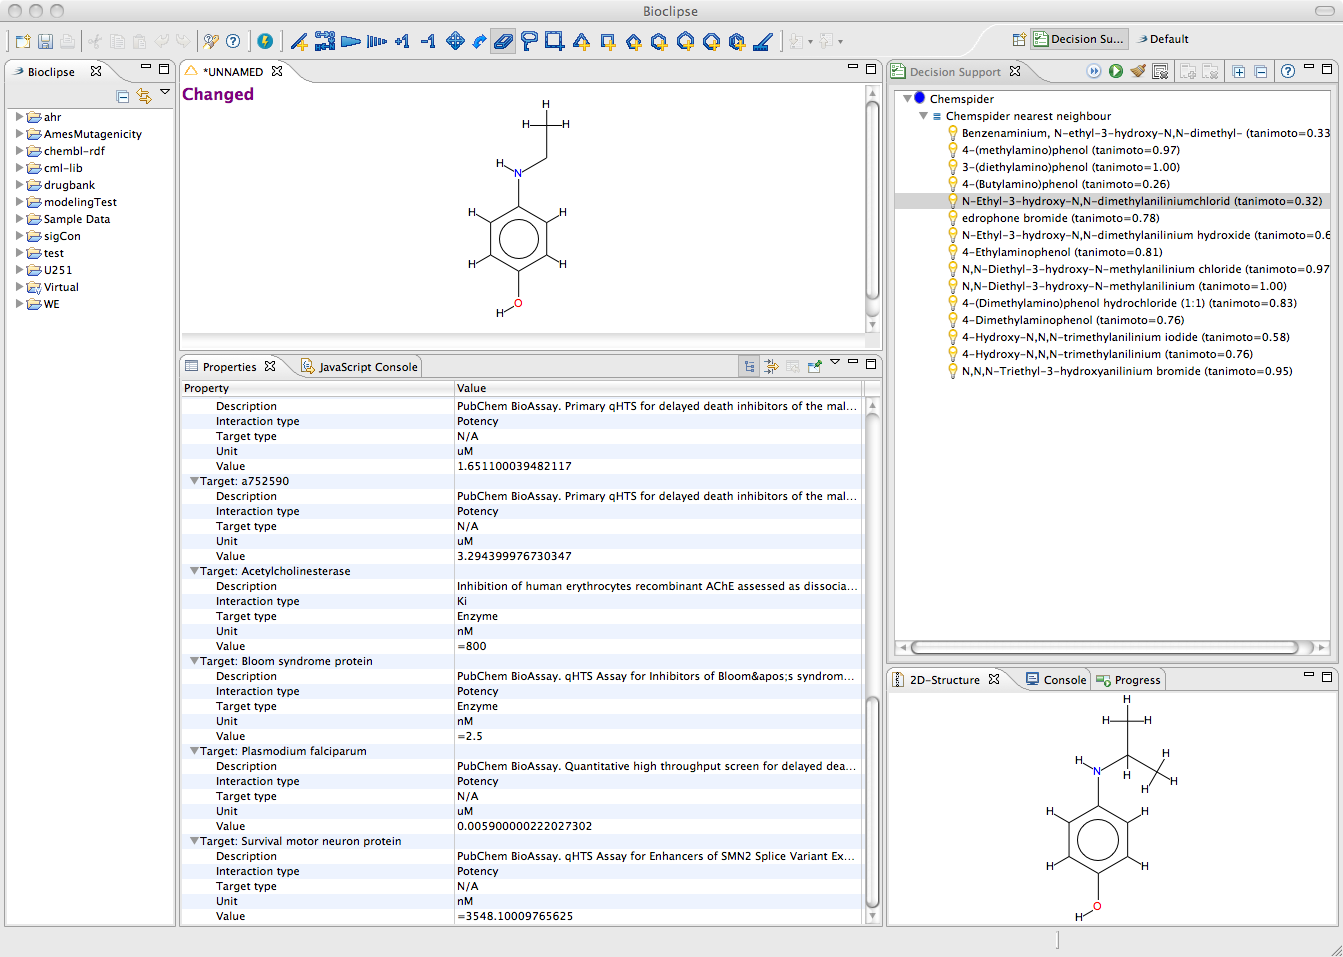
\includegraphics[width=16cm]{bioclipse-ds.png}
		\newline
		\caption[wee]{Screnshot from Bioclipse Decision Support with results from a ChemSpider + ChEMBL-RDF search. The top middle canvas contains the query structure, the top right canvas shows the near neighbors in ChemSpider (via a similarStructure search), the lower right shows the chemical structure for the selected compound in the top right canvas, and the lower center canvas shows the found interactions for this compound.}
	\label{fig:bioclipse-ds}
		\end{center}
\end{figure*}


\subsection{Chem2Bio2RDF}

David/Bin: Chem2Bio2RDF

\subsection{Compound Selectivity}

NOTE: May want to exclude this Use Case as query has not successful run yet, keeps causing virtuoso 
to timeout or run out of memory. Currently playing with local server setup to get query to run.

Designing a molecule, which is selective to one target over another will often be considered a 
successful outcome in a drug design process. If the target in question is a protein, it is easy
to understand that as sequence identity amongst residues, which contribute to potential small 
molecule binding sites remains high so does the issue of selectivity. That is, the molecule being 
designed may also bind to the equivalent binding site in the  closely related protein 
target and may lead to undesirable consequences. The ChEMBL data model links molecules to 
targets using different activity types recorded in the literature. Using activity types, 
which act as a measure of binding affinity, such as IC50 or Ki and applying activity value cuts
offs it is possible to identify molecules which have higher binding affinity to certain targets 
compared to others. Taking this one step further it is possible to identify a set molecules, 
which have a high affinity to protein A (e.g. IC50 value < 50nM) and low affinity to protein 
B (e.g. IC50 value > 200nM). 

The following SPARQL query identifies a set of molecules, which based on data curated from the 
literature and stored in the ChEMBL-RDF data model, selectively bind Human Cyclin-Dependent Kinase 2 
(UniProt: P24941) over Human Cyclin-Dependent Kinase 4 (UniProt: P11802). 

NOTE: Query should return 65 molecules

\begin{tiny}
\begin{verbatim}
select distinct ?molecule WHERE 
{ 
  ?assay ?p chembl:Assay ;
  chembl:hasTarget ?target .
  ?activity ?p chembl:Activity ;
  chembl:forMolecule ?molecule ;
  chembl:onAssay ?assay ;
  chembl:type ?type ;
  chembl:standardUnits ?unit ;
  chembl:standardValue ?value;
  chembl:relation ?relation
  FILTER (
    ?type = "IC50"  &&
    ?unit = "nM"    &&
    ?value  < 50    &&
    ?relation = "="
  ) .
  ?target ?p chembl:Target;
  dc:identifier ?id
  FILTER (
    ?id = "uniprot:P24941"
  ) .
  { 
    select ?molecule WHERE 
    {
      ?assay ?p chembl:Assay ;
      chembl:hasTarget ?target .
      ?activity ?p chembl:Activity ;
      chembl:forMolecule ?molecule ;
      chembl:onAssay ?assay;
      chembl:type ?type ;
      chembl:standardUnits ?unit ;
      chembl:standardValue ?value ;
      chembl:relation ?relation
      FILTER (
        ?type = "IC50"  &&
        ?unit = "nM"    &&
        ?value  > 200   &&
        ?relation = "="
      ) .
      ?target ?p chembl:Target;
      dc:identifier ?id
      FILTER (
        ?id = "uniprot:P11802"
      ) .
    }
  }
}
\end{verbatim}
\end{tiny}

Analysis on the set of molecules returned by this query can be used to help identify small 
molecule features, which may increase target-binding specificity. For queries which link 
small molecules to targets, by traversing bioactivity data in the ChEMBL database, it is 
also important to consider the parameters associated with the assay to target mappings. 
These additional parameters include a relationship type, a multi flag (for poorly defined
targets) a complex flag (for protein complex targets) and a curation level. These different 
factors are summarized in the ChEMBL confidence score, which ranges from 9 (direct single 
protein target) to 0 (uncurated). In order to return the largest possible dataset, the 
confidence score has been ignored in this example compound selectivity use case.

\section{Discussion}

While we show here that the RDF version of the ChEMBL data is very useful, the current RDF triples are by no means static: ChEMBL-RDF
will keep evolve, following new developments in the Linked Open Data world. For example, it is likely that over time we will link out
to more Linked Data resources. More importantly, we wish to adopt more common ontologies, of which the BioAssay Ontology is planned
to be the next~\cite{Visser2011}. These steps will make the ChEMBL-RDF triples even more interoperable.

\section{Acknowledgements}

Tim Hodson and Zach Beauvais of Kasabi and A. L\"ovgren at the BMC Computing Department at Uppsala University for their
support. OS acknowledges funding from the Swedish VR (2011-6129) and eSSENCE.

The data in ChEMBL is made available by funding from the Wellcome Trust [086151/Z/08/Z]

\bibliography{article}

%%%%%%%%%%% The bibliography starts:
%\begin{thebibliography}{9}
%
%\bibitem{r1}
%
%\bibitem{r2}
%
%\end{thebibliography}

\end{document}
